% fig5_gauge_symmetry.tex
%
% Why concentration cannot separate the iron source from the iron sink, drawn as the geometry it
% actually is: a one-parameter multiplicative gauge symmetry.
%
% The claim this figure is allowed to make, per
% docs/findings/2026-07-30_iron_closure_ude_is_a_gauge_symmetry.md section 5:
%   MAY say  - the degeneracy is a one-parameter multiplicative gauge symmetry
%            - the LEVEL of the sink is unidentified from concentration, and no multiplicative
%              closure can change that
%            - the SHAPE survives the gauge and is a legitimate estimand
%   MAY NOT  - "breaking the degeneracy", "recovering the scavenging rate",
%              "learning the iron closure from data"
% The wording on this figure is chosen to stay on the right side of that line.
%
% Left panel  : the valley. Concentration contours run ALONG it, so concentration slides freely.
% Right panel : what each observable does. A flux observation cuts ACROSS; another concentration
%               does not.
%
% ---------------------------------------------------------------------------------------
% TECHNIQUE ADAPTED, WITH THANKS:
%   curved surface via to[out=,in=] Bezier segments with a gradient fill, after
%     tikz.net "Manifold"        https://tikz.net/manifold/
%   palette mixed toward black, one hue -> text/draw/fill triple, after
%     tikz.net "Neural networks" https://tikz.net/neural_networks/
% ---------------------------------------------------------------------------------------
%
%   pdflatex fig5_gauge_symmetry.tex
%
\documentclass[tikz,border=10pt]{standalone}
\usetikzlibrary{arrows.meta,positioning,calc,fit,backgrounds,decorations.pathreplacing}

\colorlet{myblue}{blue!80!black}
\colorlet{mygreen}{green!55!black}
\colorlet{myorange}{orange!85!black}
\colorlet{myred}{red!75!black}
\colorlet{myink}{black!78}

\begin{document}
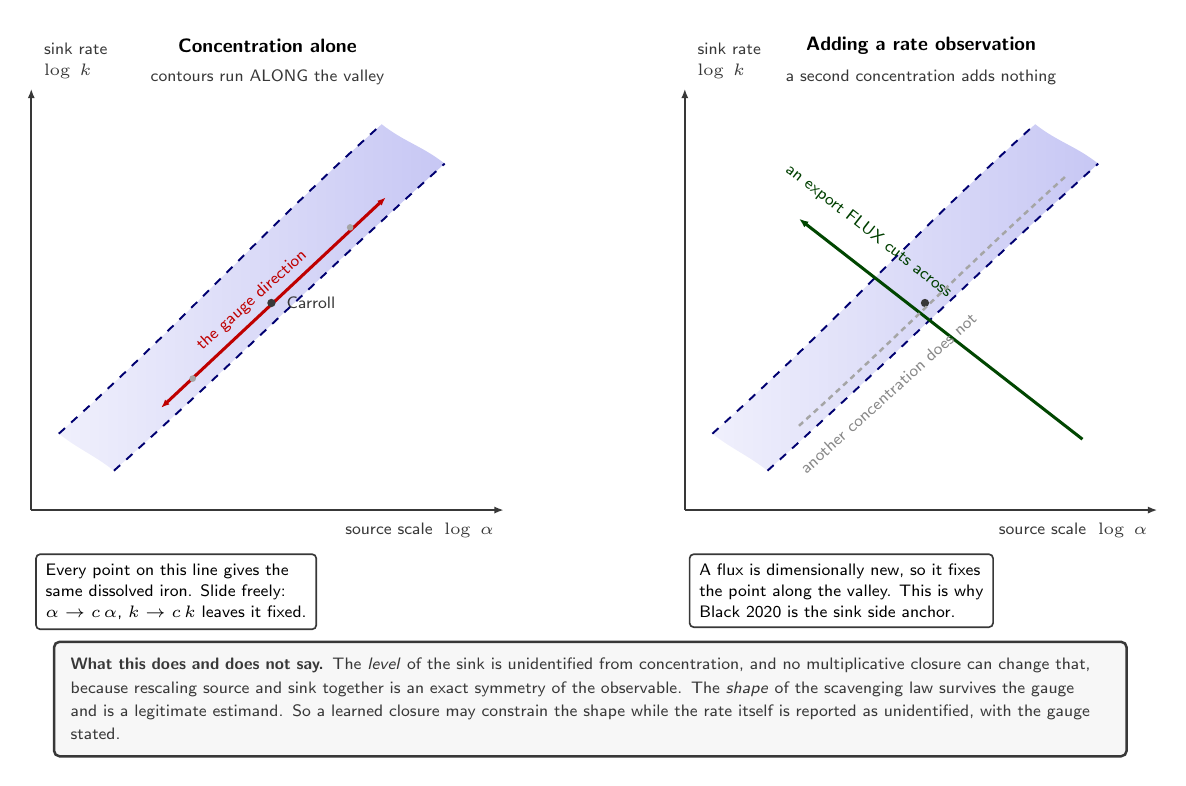
\begin{tikzpicture}[
  font=\sffamily,
  head/.style ={font=\sffamily\bfseries\scriptsize, text=black, align=center},
  note/.style ={font=\sffamily\fontsize{6.2}{7.6}\selectfont, text=myink, align=center},
  ax/.style   ={draw=myink, line width=0.6pt, -{Latex[length=3.4,width=2.6]}},
  iso/.style  ={draw=myblue!55!black, line width=0.7pt},
  gaugearr/.style={draw=myred, line width=1.1pt,
                   {Latex[length=3,width=2.4]}-{Latex[length=3,width=2.4]}},
  cut/.style  ={draw=mygreen!50!black, line width=1.1pt, -{Latex[length=3.4,width=2.6]}},
  chip/.style ={draw=myink, line width=0.6pt, rounded corners=1.5pt, fill=white,
                inner sep=3.5pt, font=\sffamily\fontsize{6.2}{7.6}\selectfont, align=left},
]

% ==================================================== LEFT: the valley
\begin{scope}
  % the degenerate valley: a soft band running diagonally. Bezier outline, gradient fill, so the
  % floor of the valley reads as flat rather than as a line.
  \shade[left color=myblue!6, right color=myblue!22, draw=none]
    (0.15,0.15) to[out=42, in=222] (4.35,4.05)
                to[out=142, in=322] (3.55,4.55)
                to[out=222, in=42]  (-0.55,0.62) to[out=322,in=142] cycle;

  \draw[iso, dashed] (0.15,0.15) to[out=42, in=222] (4.35,4.05);
  \draw[iso, dashed] (-0.55,0.62) to[out=42, in=222] (3.55,4.55);

  % axes
  \draw[ax] (-0.9,-0.35) -- (5.1,-0.35) node[below left=1pt and 0pt, note] {source scale\ \ $\log\ \alpha$};
  \draw[ax] (-0.9,-0.35) -- (-0.9,5.0)  node[above right=0pt and 1pt, note, align=left] {sink rate\\$\log\ k$};

  % the gauge direction: you can slide along the valley and nothing observable changes
  \draw[gaugearr] (0.75,0.95) -- (3.6,3.62);
  \node[note, text=myred, rotate=42, anchor=south] at (2.05,2.15) {the gauge direction};

  % Carroll sits somewhere on it, and so does every other point
  \fill[myink] (2.15,2.28) circle (1.5pt);
  \node[note, right=2pt of {(2.15,2.28)}, anchor=west] {Carroll};
  \fill[myink!45] (1.15,1.32) circle (1.2pt);
  \fill[myink!45] (3.15,3.24) circle (1.2pt);

  \node[head] at (2.1,5.55) {Concentration alone};
  \node[note] at (2.1,5.15) {contours run ALONG the valley};

  \node[chip, anchor=north west] at (-0.85,-0.9)
    {Every point on this line gives the\\same dissolved iron. Slide freely:\\
     $\alpha \to c\,\alpha$, $k \to c\,k$ leaves it fixed.};
\end{scope}

% ==================================================== RIGHT: what each observable does
\begin{scope}[xshift=8.3cm]
  \shade[left color=myblue!6, right color=myblue!22, draw=none]
    (0.15,0.15) to[out=42, in=222] (4.35,4.05)
                to[out=142, in=322] (3.55,4.55)
                to[out=222, in=42]  (-0.55,0.62) to[out=322,in=142] cycle;
  \draw[iso, dashed] (0.15,0.15) to[out=42, in=222] (4.35,4.05);
  \draw[iso, dashed] (-0.55,0.62) to[out=42, in=222] (3.55,4.55);

  \draw[ax] (-0.9,-0.35) -- (5.1,-0.35) node[below left=1pt and 0pt, note] {source scale\ \ $\log\ \alpha$};
  \draw[ax] (-0.9,-0.35) -- (-0.9,5.0)  node[above right=0pt and 1pt, note, align=left] {sink rate\\$\log\ k$};

  % a FLUX observation cuts across the valley
  \draw[cut] (4.15,0.55) -- (0.55,3.35);
  % label rides the UPPER-LEFT end of the flux line, so it clears the parallel-concentration
  % label below. Both sat mid-line in an earlier draft and crossed each other.
  \node[note, text=mygreen!45!black, rotate=-38, anchor=south] at (1.30,3.02)
    {an export FLUX cuts across};

  \fill[myink] (2.15,2.28) circle (1.5pt);

  % another concentration does not
  \draw[draw=myink!45, line width=0.9pt, dash pattern=on 2pt off 1.6pt]
    (0.55,0.72) to[out=42, in=222] (3.95,3.9);
  \node[note, text=myink!60, rotate=42, anchor=north] at (1.55,1.28)
    {another concentration does not};

  \node[head] at (2.1,5.55) {Adding a rate observation};
  \node[note] at (2.1,5.15) {a second concentration adds nothing};

  \node[chip, anchor=north west] at (-0.85,-0.9)
    {A flux is dimensionally new, so it fixes\\the point along the valley. This is why\\
     Black 2020 is the sink side anchor.};
\end{scope}

% ==================================================== what survives, stated carefully
\node[draw=myink, line width=0.9pt, rounded corners=2pt, fill=black!3,
      align=left, inner sep=6pt, font=\sffamily\fontsize{6.4}{8.4}\selectfont, text=myink,
      text width=13.2cm] at (6.2,-2.75)
  {\textbf{What this does and does not say.} The \emph{level} of the sink is unidentified from
   concentration, and no multiplicative closure can change that, because rescaling source and
   sink together is an exact symmetry of the observable. The \emph{shape} of the scavenging law
   survives the gauge and is a legitimate estimand. So a learned closure may constrain the shape
   while the rate itself is reported as unidentified, with the gauge stated.};

\end{tikzpicture}
\end{document}
